In this chapter we will walk through three simplified binary PFC models. The
first is the original binary PFC model, which, while highly successful at
modelling a few important phenomena is ultimately limited in scope. The second
is the binary structural phase field crystal, or binary XPFC which was
successful in modelling a broad spectrum of crystalline structures, but was
limited in its ability of model liquid instablilities and a variety of phase
diagrams. Finally, we'll see a new contribution to which we will call the
regular phase field crystal model which is successful in modeling a broad
spectrum of invariant binary reactions and crystalline structures. 

All binary PFC models begin with a multicomponent variant of the approximate
free energy functional established in Chapter \ref{fundamentals},
%
\begin{align}
    \label{binary_cdft_free_energy}
    \beta\F[\A, \B] &= \sum_{i=A, B} \int \mathrm{d}r 
        \,\rho_i(r) \ln\l(\f{\rho_i(r)}{\rho_i^0}\r) 
        - (1 - \beta\mu_i^0)\Delta\rho_i(r)\\
    &- \f{1}{2} \sum_{i,j=A, B} \Delta\rho_i(r) \ast C^{(2)}_{ij}(r, r^\prime) 
        \ast \Delta\rho_j(r^\prime). \nonumber
\end{align}
%
It is convenient to change variables to a dimensionless total density, $n(r)$
and local concentration, $c(r)$,
%
\begin{gather}
    n(r) = \f{\Delta \rho}{\rho_0} = \f{\Delta\A + \Delta\B}{\A^0 + \B^0} \\
    c(r) = \f{\B}{\rho} = \f{\B}{\A + \B}.
\end{gather}
%
Scaling out a factor of the total reference density, $\rho_0$ we can break the
free energy functional in these new variables into three parts,
%
\begin{equation}
    \label{binary_total_free_energy}
    \f{\beta\F[n, c]}{\rho_0} = \f{\beta\F_{id}[n]}{\rho_0} 
        + \f{\beta\F_{mix}[n, c]}{\rho_0}
        + \f{\beta\F_{ex}[n, c]}{\rho_0},
\end{equation}
%
Where,
%
\begin{gather}
    \label{binary_ideal}
    \f{\beta\F_{id}[n]}{\rho_0} =
        \int \mathrm{d}r \,\l\lbrace (n(r) + 1)\ln(n(r) + 1) 
        - (1 - \beta\mu^0)n(r) \r\rbrace \\
    \label{binary_mixing}
    \f{\beta\F_{mix}[n, c]}{\rho_0} =
        \int \mathrm{d}r \,\l\lbrace (n(r) + 1)\l( 
            c\ln\l(\f{c}{c_0}\r) + (1-c)\ln\l(\f{1-c}{1-c_0}\r) \r)\r\rbrace, 
\end{gather}
%
And, if we assume the local concentration $c(r)$ varies over much longer length
scales than the local density $n(r)$,
%
\begin{align}
    \label{binary_excess}
    \f{\beta\F_{ex}[n, c]}{\rho_0}
        = &-\f{1}{2} n(r) \ast \l[ 
            C_{nn}(r, r^\prime) \ast n(r^\prime) 
          + C_{nc}(r, r^\prime) \ast \Delta c(r^\prime)\r] \\
        &-\f{1}{2} \Delta c(r) \ast \l[
            C_{cn}(r, r^\prime) \ast n(r^\prime) 
          + C_{cc}(r, r^\prime) \ast \Delta c(r^\prime)\r]. \nonumber
\end{align}
%
We have introduced $\mu_0$ as the total chemical potential of the reference
mixture, $c_0 = \B^0 / \rho_0$ as the reference concentration and $\Delta c(r)
= c(r) - c_0$ as the deviation of the concentration from the reference.  The
$n-c$ pair correlation introduced in the excess free energy are,
%
\begin{align}
    C_{nn} &= \rho_0\l(c^2 C_{BB} + (1 - c)^2C_{AA} + 2c(1-c)C_{AB}\r) \\
    C_{nc} &= \rho_0\l(c C_{BB} - (1 - c) C_{AA} + (1 - 2c)C_{AB}\r) \\
    C_{cn} &= C_{nc} \\
    C_{cc} &= \rho_0\l(C_{BB} + C_{AA} - 2 C_{AB}\r)
\end{align}
%
Explicit calculations can be found in Appendix \ref{binary_correlations}.
Differences in the various simplified binary PFC theories stem from differing
approximations of the terms in the free energy stated in equation
\ref{binary_total_free_energy}.

%%%%%%%%%%%%%%%%%%%%%%%%%%%%%%%%%%%%%%%%%%%%%%%%%%%%%
\section{Original Binary Phase Field Crystal Model} %
%%%%%%%%%%%%%%%%%%%%%%%%%%%%%%%%%%%%%%%%%%%%%%%%%%%%%

In the original simplified binary PFC theory, all terms in the free energy are
expanded about $n(r) = 0$ and $c(r) = c_0$ (ie., about their reference states).
For the ideal free energy this results in a polynomial truncated to fourth
order,
%
\begin{equation}
    \label{ideal_expansion}
    \f{\beta\F_{id}[n]}{\rho_0} = \integrate{r}
    \l\lbrace \f{n(r)^2}{2} - \f{n(r)^3}{6} + \f{n(r)^4}{12} \r\rbrace.
\end{equation}
%
The linear term is dropped due to invariance in the equations of motion. If we
assume for simplicity of demonstration $c0 = 1/2$, the free energy of mixing
becomes a simple fourth order polynomial as well,
%
\begin{equation}
    \f{\beta\F_{mix}[n, c]}{\rho_0} = \integrate{r} \l\lbrace
       2\Delta c(r)^2 + \f{4\Delta c(r)^4}{3}
    \r\rbrace.
\end{equation}
%
Linear couplings to $n(r)$ are dropped by assuming, as we already have, that
the concentration field varies on a much longer length scale than the total
density and noting that the total density is defined about its average. This
argument can also be applied the linear couplings to $n(r)$ in the excess free
energy term which leaves only the $C_{nn}$ and $C_{cc}$ terms. Finally, these
two terms are approximated with a gradient expansions of the correlation
functions,
%
\begin{gather}
    C_{nn}(r, r^\prime) = \d(r - r^\prime)\l(
        \alpha + \beta \nabla^2 + \gamma \nabla^4 + \dots\r), \\
    C_{cc}(r, r^\prime) = \d(r - r^\prime)\l(
        \epsilon + \xi \nabla^2 + \dots\r).
\end{gather}
%
The expansion parameters, $\alpha, \beta,$ and $\gamma$ are all dependent on
temperature and concentration. We are required to expand $C_{nn}$ to fourth
order because, as noted in chapter \ref{dft_of_freezing} the peak of the direct
correlation function in Fourier space is the driving force for solidification.
The concentration field is correlated over a longer length scale implying that
only the short wavevectors are important in $C_{cc}$ so we can expand just to
quadratic order.

Gathering terms the resulting free energy functional for the original simplified
binary PFC model\footnote{The orignal simplified binary PFC model was
expressed using slightly different variables. We expand in $\Delta c(r)$ here to 
facilitate comparison with other theories} is,
%
\begin{align}
    \f{\beta\F[n, c]}{\rho_0} &= \integrate{r} \l\lbrace 
        \f{1}{2} n(r) \l( 1 - \alpha - \beta\nabla^2 - \eta\nabla^4 \r) n(r)
      - \f{n(r)^3}{6} + \f{n(r)^4}{12} \r\rbrace \\
    &+ \integrate{r} \l\lbrace
        \f{1}{2} \Delta c(r) \l( 4 - \epsilon - \xi\nabla^2 \r) \Delta c(r) 
      + \f{4 \Delta c(r)^4}{3} \r\rbrace. \nonumber
\end{align}
%

The strength of the original simplified binary PFC model is that is retains
most of the important physics of binary alloys in a very reduced theory. For
instance, the simplified model is capable of describing the equilibrium phase
diagrams of both eutectic alloys alloys and materials with a solid state
spinodal / liquid minimum.  Supplied with a diffusive equation of motion the
simplified model can model an impressive diversity of dynamic phenomena
including eutectic growth, phase segregation, dendritic growth, dislocation
motion in solid state spinodal coarsening and epitaxial growth.

The major limitation of the original simplified model is that the gradient
expansion of the density-density correlation function gives only a crude
control over the structures that will be formed. In fact, as this theory only
controls a single peak in Fourier space it can only solidify into the fcc phase
[{\color{ForestGreen} check this is the case for the original theory}]. As
noted in chapter \ref{dft_of_freezing}. The ability to solidify into an
arbitrary structure demands control of value of the density-density correlation
function at all reciprocal lattice vectors.

A second limitation of the original simplified model is that it is local in
concentration. This means that realistic phase diagrams from 0 to 100\%
concentration cannot be produced, only local phase diagrams around the
reference concentration that was expanded about. To construct these global
phase diagrams we require the entire free energy of mixing term in equation
\ref{binary_mixing}.

%%%%%%%%%%%%%%%%%%%%%%%%%%%%%%%%%%%%%%%%%%%%%%%%%%%%%%%
\section{Binary Structural Phase Field Crystal Model} %
%%%%%%%%%%%%%%%%%%%%%%%%%%%%%%%%%%%%%%%%%%%%%%%%%%%%%%%

The binary structural phase field crystal theory (XPFC) seeks to remedy the two
short comings of the original simplified model. That is, it seeks to construct
realistic phase diagrams for binary systems and seeks to reproduce a variety 
of crystal lattice structure. We'll begin with a derivation of the theory and
compare with the original model.

First, the ideal free energy is expanded in precisely the same manner resulting
in the same fourth order polynomial,
%
\begin{equation}
    \f{\beta\Delta\F_{id}[n]}{\rho_0} = \integrate{r}
        \l\lbrace \f{n(r)^2}{2} - \eta \f{n(r)^3}{6} + \chi\f{n(r)^4}{12}
        \r\rbrace. \tag{\ref{ideal_expansion} revisited}
\end{equation}
%
The free energy of mixing is left unexpanded but an overall scale $\omega$ is
added to fit the mixing term away from the reference concentration,
%
\begin{equation}
    \f{\beta\F_{mix}[n, c]}{\rho_0} =
        \integrate{r} \l\lbrace \omega (n(r) + 1)\l( 
            c\ln\l(\f{c}{c_0}\r) + (1-c)\ln\l(\f{1-c}{1-c_0}\r) \r)\r\rbrace. 
\end{equation}
%
This unexpanded free energy of mixing will lead to more accurate global phase
diagrams. The excess free energy is approximated using the similar assumptions
as in the original model (linear couplings are dropped), but the density-density
correlation function is not expanded. Greenwood \textit{et al} all assumed that
the $k=0$ mode of the concentration-concentration correlation function was zero
leaving only the quadratic term in the expansion,
%
\begin{equation}
    C_{cc}(r, r^\prime) = \d(r - r^\prime)\alpha \nabla^2.
\end{equation}
%
Grouping terms together, the complete free energy functional for the binary XPFC
model is,
%
\begin{align}
    \f{\beta\Delta\F[n, c]}{\rho_0} &= \integrate{r} \l\lbrace
        \f{1}{2} n(r) \l(1 - C_{nn}(r, r^\prime)\r) \ast n(r^\prime)
        - \eta \f{n^3}{6} + \chi \f{n^4}{12} \r\rbrace \\
        &+ \integrate{r}\l\lbrace
            \f{1}{2}\l\vert \nabla c(r) \r\vert^2 + \omega f_{mix}(r)
            \r\rbrace. \nonumber
\end{align}
%
Where $f_{mix}(r)$ is the local free energy density of mixing,
%
\begin{equation}
    f_{mix}(r) = \l(n(r) + 1\r)\l( 
            c(r)\ln\l(\f{c(r)}{c_0}\r) + (1-c(r))\ln\l(\f{1-c(r)}{1-c_0}\r) \r).
\end{equation}
%

%%%%%%%%%%%%%%%%%%%%%%%%%%%%%%%%%%%%%%%%%%%%%%
\subsection{Modelling Correlation Functions} %
%%%%%%%%%%%%%%%%%%%%%%%%%%%%%%%%%%%%%%%%%%%%%%

The key insight made by the XPFC model the that, the density-density correlation 
function can be modelled in such a way as to control the crystall lattice structure
targetted under cooling and to target different structures at different concentrations.
Note that the density-density correlation function as the form of a linear combination
of interpolating functions in concentration, $\zeta(c)$, multiplied by bare correlation
functions $C(r, r^\prime)$,
%
\begin{equation}
    C_{nn}(r, r^\prime; c) = \sum_i \zeta_i(c) C_i(r, r^\prime)
\end{equation}
%
In the exact theory, for example, we have,
%
\begin{gather}
    \zeta_{AA}(c) = \rho_0 (1 - c^2), \\
    \zeta_{AB}(c) = \rho_0 c (1 - c ), \\
    \zeta_{BB}(c) = \rho_0 c^2.
\end{gather}
%
Each interpolating function, $\zeta_i(c)$, defines a domain of validity for its
associated correlation function $C_i(r, r^\prime)$. This suggests that we might
model any density-density correlation function using this general structure:
the set of correlation function $C_i(r, r^\prime)$ enumerate the various
structures that may manifest themselves and the associated interpolation
functions $\zeta_i(c)$ define the concentrations over which these correlations
are valid.

As a simple example we wanted to construct a simple model of the silver-cupper
eutectic alloy system, we might start with some model correlation function for
pure silver, $C_\alpha(r, r^\prime)$, and for pure copper, $C_\beta(r,
r^\prime)$. These two structures, the silver rich $\alpha$ phase and the copper
rich $\beta$ phase, are the only two relevent crystalline structures in the
system so to build the full density-density correlation function we just need
to choose interpolating functions for each. Following Greenwood \textit{et al}
for example, we might choose,
%
\begin{gather}
    \zeta_\alpha(c) = 1 - 3c^2 + 2c^3, \\
    \zeta_\beta(c) = 1 - 3 (1 - c)^2 + 2(1 - c)^3.
\end{gather}
%

This leaves the question of how to develop model correlation functions for any
particular crystalline lattice of interest. This problem is also anwsered by
the XPFC framework. Originally delineated for pure systems, the XPFC method for
constructing correlation functions is strongly influenced by the methods
developed by Ramakrishnan. In particular this means that, given that the
driving force for solidification is the of value direct correlation function at
the reciprocal lattice vectors, we need a model correlation function that
controls these parameters specifically. We can acheive this with Gaussian peaks
centred at the reciprocal lattice vector positions,
%
\begin{equation}
    C_i(r, r^\prime) = \sum_{\alpha} e^{\f{T}{T_i^0}}
        e^{ - \f{(k - k_i)^2}{2\sigma_i^2}}
\end{equation}
%
Where, as in chapter \ref{dft_of_freezing}, the index $\alpha$ runs over
families of point group equivalent reciprocal lattice vectors. The temperature
dependent prefactors $e^{T / T_i^0}$ give the correct temperature scaling of
the amplitudes close to the melting point\footnote{The original XPFC works used
a phenomonological prefacter with $e^{T^2 / C_i}$ for a constant $C_i$. This
choice is inspired by harmonic analysis in the solid phase and the Debye-Waller
factor} as discussed by \cite{ALSTER17}.

The advantages of the XPFC simplified binary model are two fold: realistic 
phase diagrams and modelling a variety of crystalline lattices. While the
former is relatively cosmetic the latter allows for the examination of 
guininely novel systems in comparison with the original simplified model. For
example the binary XPFC model as been used to study, peritectic systems, 
ordered crystals, [{\color{ForestGreen} find refs and list of applications}]
\cite{GREENWOOD11, ALSTER17}. 

Unfortunately, by assuming that the $k=0$ mode of the concentration-concentration
correlation function is zero the XPFC model restricts the its free energy of
mixing to an ideal model of mixing. This model of mixing includes only entropic
contributions to the free energy. This means that the sole driving force for 
phase seperation is elastic energy as the heat of mixing is always positive (
{\color{ForestGreen} right? I always mess up this convention}). This can be a
limitation on modelling a variety of binary alloy systems, for instance both
monotectic and syntectic systems cannot be modelled without a negative heat
of mixing. More subtly, even eutectic systems have a negative heat of mixing deep
below the eutectic point as the metastable liquid has a spinodal point. Problems 
such as the stability of nanocrystalline binary alloys require an examination of
the balance of elastic energies and bulk mixing free energy \cite{murdoch}.

%%%%%%%%%%%%%%%%%%%%%%%%%%%%%%%%%%%%%%%%%%%%%
\section{Regular Phase Field Crystal Model} %
%%%%%%%%%%%%%%%%%%%%%%%%%%%%%%%%%%%%%%%%%%%%%

The regular phase field crystal model is a simplified model that aims to combine 
the positive aspects of the XPFC and original simplified models together. The 
original PFC model uses an regular model of mixing so both enthalpic and entropic 
contribution to the free energy of mixing are considered. This is acheived by
assuming there is a $k=0$ contribution in the gradient expansion of the 
concentration-concentration correlation function. If we add this simple component
to the development of the XPFC free energy functional we find one additional term
that gives an enthaly of mixing,
%
\begin{align}
    \f{\beta\Delta\F[n, c]}{\rho_0} &= \integrate{r} \l\lbrace
        \f{1}{2} n(r) \l(1 - C_{nn}(r, r^\prime)\r) \ast n(r^\prime)
        - \eta \f{n^3}{6} + \chi \f{n^4}{12} \r\rbrace \\
        &+ \integrate{r}\l\lbrace
            \f{1}{2}\l\vert \nabla c(r) \r\vert^2 + \omega f_{mix}(r)
            \r\rbrace. \nonumber
\end{align}
%
Where the local free energy density of mixing, $f_{mix}$ is now,
%
\begin{equation}
    f_{mix}(r) = \l(n(r) + 1\r)\l( 
            c(r)\ln\l(\f{c(r)}{c_0}\r) + (1-c(r))\ln\l(\f{1-c(r)}{1-c_0}\r) \r) + 
            \f{1}{2} \epsilon (c - c_0)^2.
\end{equation}
%
The simplicity the temperature dependence if the parameter $\epsilon$ is taken to be
linear about the spinodal temperature $T_c$,
%
\begin{equation}
    \epsilon(T) = -4 + \epsilon_0(T - T_c).
\end{equation}

%%%%%%%%%%%%%%%%%%%%%%%%%%%%%%%%%%%%%
\subsection{Equilibrium Properties} %
%%%%%%%%%%%%%%%%%%%%%%%%%%%%%%%%%%%%%

Here we'll explore the flexibility of the simplified regular PFC model in
describing various material phase diagrams in binary systems.

%%%%%%%%%%%%%%%%%%%%%%%%%%%%%%%%%%%%%%%%
\subsubsection{Eutectic Phase Diagram} %
%%%%%%%%%%%%%%%%%%%%%%%%%%%%%%%%%%%%%%%%

While previous PFC models have shown that elastic energy is a sufficient
driving force for eutectic solidification our simplified regular model allows
for the examination of the role enthalpy of mixing can play in eutectic solids.
For instance, Murdoch and Schuh noted that in nanocrystalline binary alloys,
while a positive enthaply of segregation can stabilize against grain growth via
solute segregation at the grain boundary, if the enthaply of mixing becomes too
large this effect can be negated by second phase formation or even macroscopic
phase seperation\cite{MURDOCH13}. 

To specialize our simplified regular model to the case of the binary eutectic
we must choose an appropriate model for the correlation function. Choosing an
$\alpha$ phase around $c = 0$ and $\beta$ phase around $c = 1$, we can recover
the pair correlation function used in the binary XPFC with a
particular choice of window functions: 
%
\begin{align}
   \zeta_\alpha(c) &= 2c^3 - 3c^2 + 1 \\
   \zeta_\beta(c) &= \zeta_\alpha(1 - c).
\end{align}
%
Should we choose, for example, an $\alpha$ and $\beta$ phase with 2 dimensional
hexagonal lattices, differing only by lattice constants, we can produce a phase
diagram like that in Fig. \ref{eutectic}.  

\begin{figure}[h]
    \centering	
    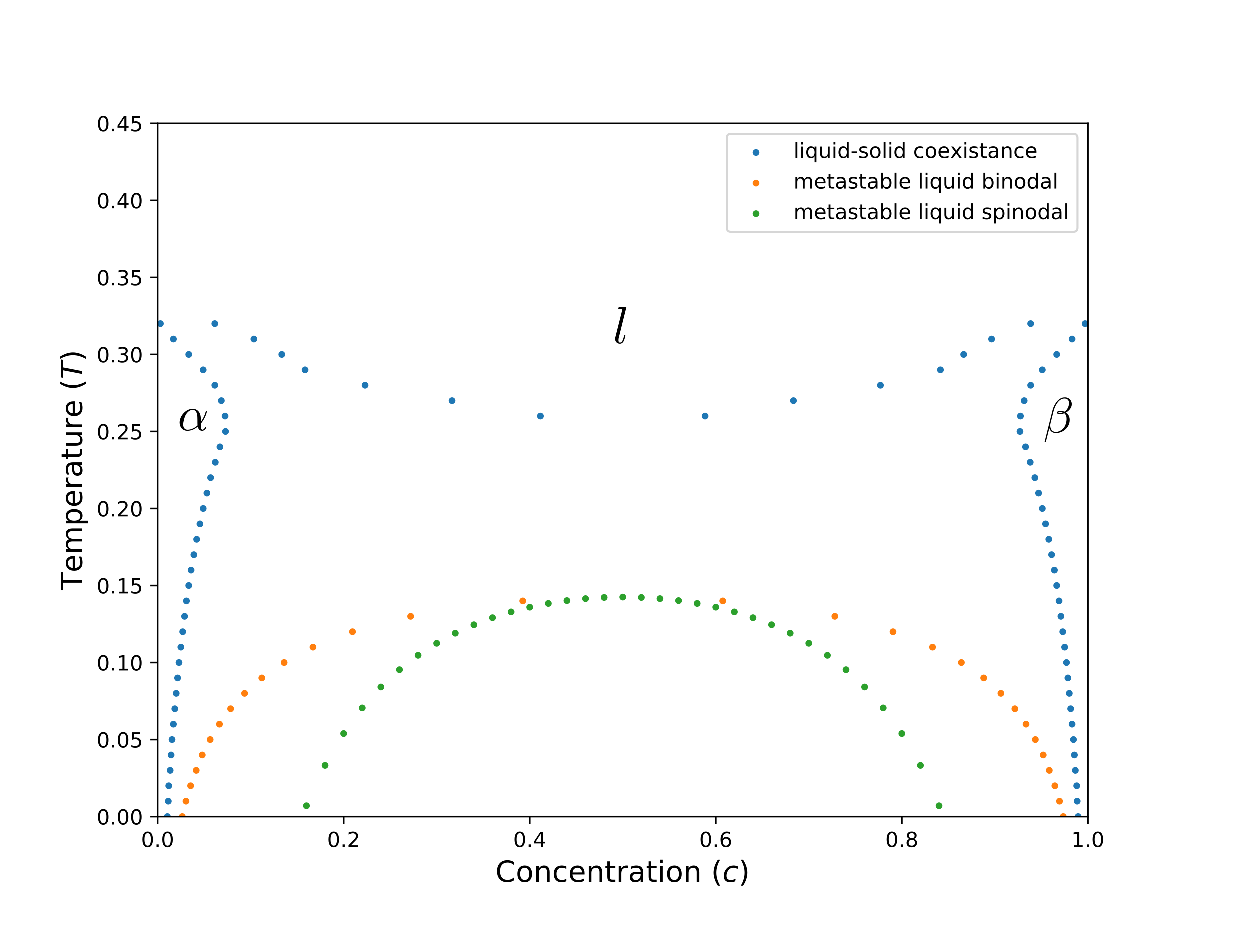
\includegraphics[scale=0.7]{eutectic}
    \caption{
        \label{eutectic} Eutectic phase diagram triangle $\alpha$ and $\beta$
        phases. The free energy parameter are $\eta = 2$, $\chi = 1$,
        $\omega=0.30$, $\epsilon_0 = 3$ and $T_c = 0.01$. The parameters of the
        structure functions are $\alpha_{10\alpha} = \alpha_{10\beta} = 0.8$,
        $k_{10\alpha} = 2\pi$, $k_{10\beta} = 4\pi/\sqrt{3}$ and $T_0 = 1$
    }
\end{figure}

%%%%%%%%%%%%%%%%%%%%%%%%%%%%%%%%%%%%%%%%%
\subsubsection{Syntectic Phase Diagram} %
%%%%%%%%%%%%%%%%%%%%%%%%%%%%%%%%%%%%%%%%%

Our regular model also allows for the study of a variety of invariant binary
reactions that, to date, have not been studied using phase field crystal
models. One such reaction is the syntectic reaction. 

The syntectic reaction, $l_1 + l_2 \rightarrow \alpha $, consists of
solidification at the interface of two liquids. We can achieve this with our
model by setting the spinodal temperature, $T_c$, sufficiently high and
producing a density-density correlation function that is peaked at a
concentration below the spinodal. This can be done by choosing a window
function that is centered about an intermediate concentration, $c_\alpha$ of
the solid phase, $\alpha$. 
%
\begin{equation}
  \chi(c) = e^{- \f{(c - c_\alpha)^2}{2 \alpha_c}}
\end{equation}
%
The resulting correlation function for a hexagonal lattice in two dimensions,
for example, would be,
%
\begin{equation}
  \tilde{C}_{nn}(k; c) = 
    e^{-\f{(c - c_\alpha)^2}{2 \alpha_c}}
    e^{-\f{T}{T_0}} 
    e^{-\f{(k - k^\prime)^2}{2\alpha^2}}
\end{equation}
%
A phase diagram that produces a syntectic reaction with an appropriate choice
of parameters can be seen in Fig. \ref{syntectic}.

\begin{figure}
    \centering
	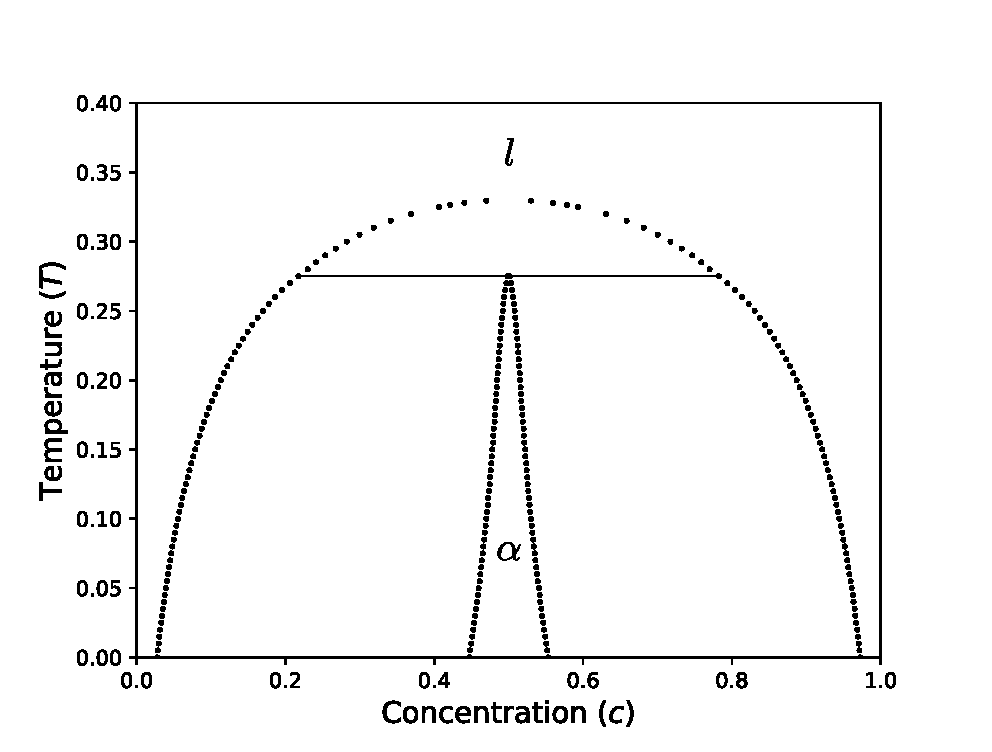
\includegraphics[scale=0.7]{syntectic.eps}
	\caption{
        \label{syntectic} Phase Diagram of Syntectic Alloy with a hexagonal
        $\alpha$ phase. The free energy parameters are $\eta=2$, $\chi=1$,
        $\omega=0.3$, $\epsilon_0 = 10$ and $T_c=0.35$. The parameters for the
        structure function are $\alpha_{10\alpha} = 0.8$, $k_{10\alpha} = 2\pi$
        and $T_0 = 1$
    }
\end{figure}

%%%%%%%%%%%%%%%%%%%%%%%%%%%%%%%%%%%%%%%%%%
\subsubsection{Monotectic Phase Diagram} %
%%%%%%%%%%%%%%%%%%%%%%%%%%%%%%%%%%%%%%%%%%

The monotectic reaction is another invariant binary reaction that has not
previously been studied using PFC models. The monotectic reaction, $l_1
\rightarrow \alpha + l_2$, consists of decomposing liquid into a solute poor
solid and solute rich liquid. To model a monotectic using our regular model we
hypothesize a solid phase at $c=0$ and set the spinondal temperature higher
than the solidification temperature. To achieve this we use a window function
peaked around $c = 0$,
%
\begin{equation}
    \chi_\alpha(c) = e^{-\f{c^2}{2\alpha_c^2}}.
\end{equation}
%
Again considering a simple hexagonal lattice for the $\alpha$ phase, we can
produce a phase diagram with a monotectic reaction with an appropriate choice
of parameters as in Fig. \ref{monotectic}.

\begin{figure}
    \centering
	\includegraphics[scale=0.7]{monotectic.eps}
	\caption{
        \label{monotectic} Phase Diagram of Monotectic Alloy with hexagonal
        $\alpha$ phase. The free energy parameters are $\eta = 2$, $\chi=1$,
        $\omega=0.3$, $\epsilon_0 = 10$, $T_c = 0.35$ and $c_0 = 0.75$. The
        parameters for the structure function are $\alpha_{10\alpha} = 0.8$,
        $k_{10\alpha} = 2\pi$ and $T_0 = 1$ and the parameter for the window
        function is $\alpha_c = 0.4$
    }
\end{figure}

%%%%%%%%%%%%%%%%%%%%%%%%%%%%%%%%%%%%%%%%%%%%%
\subsubsection{Precipitation from Solution} %
%%%%%%%%%%%%%%%%%%%%%%%%%%%%%%%%%%%%%%%%%%%%%

We can also model precipitation of nanoparticles from solution. While on its
surface the equilibrium phase diagram of a solution is that of a simple
solid-liquid coexistance, in practice the metastable features of the phase
diagram can have profound implications on the nucleation kinetics of
precipitate. As an example, precipitation from solution is a typical synthesis
technique for gold and silver nanoparticles. Recent work by Loh \textit{et al}
shows that a metastable spinodal may be playing an important role in the growth
and nucleation of gold nanoparticles under certain diffusive circumstances.

Using the regular XPFC model we can reproduce the condition of a metastable
liquid spinodal underneath the liquid-solid coexistance curve. The approach to
produce a phase diagram is the same as that of of a monotectic, with the
exception that the spinodal temperature, $T_c$, most now be sufficiently low to
be buried underneath the coexistance curve. In keeping with the concentration
being that of the solute, we'll also center the gaussian window function about
$c = 1$. An example, including metastable spinodal, can be seen in Fig.
\ref{precip}.

\begin{figure}
    \centering	
    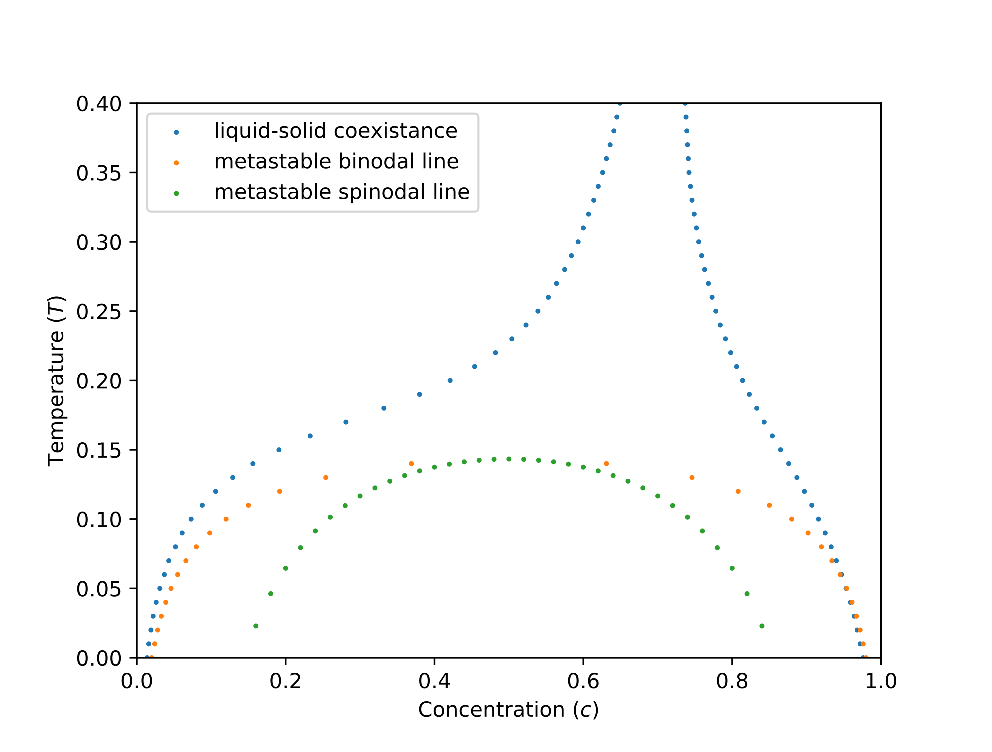
\includegraphics[scale=0.6]{solution.eps}
	\caption{
        \label{precip} Phase Diagram of Solution \color{ForestGreen} fill
        me in please!!
    }
\end{figure}


{
    \color{ForestGreen} Conclude the chapter with discussion of where what we've
    seen and lead into the discussion for the next chapter of dynamics and
    applications of this theory to more than just simple equilibrium 
    phase diagrams
}
